\part{Integrated Circuits}
\begin{nonumberframe}
    \vfill
    \centering
    \begin{beamercolorbox}[sep=8pt,center,shadow=false,rounded=true]{title}
    \usebeamerfont{title}Part I - INTEGRATED CIRCUITS\par%
    \usebeamerfont{subtitle} GUT meeting 13/01/2026
    \end{beamercolorbox}
    \vfill
\end{nonumberframe}

\section{Abstractions}
\subsection{Layers}
\begin{frame}{\insertsubsection}{\insertsection}
   % One or more splide to present the abstractions layer
   % System, Data Flow (Pipelines, Algorithm), Modules, Netlist Gate-level, Physical design, Waffer
    \begin{figure}
        \centering
        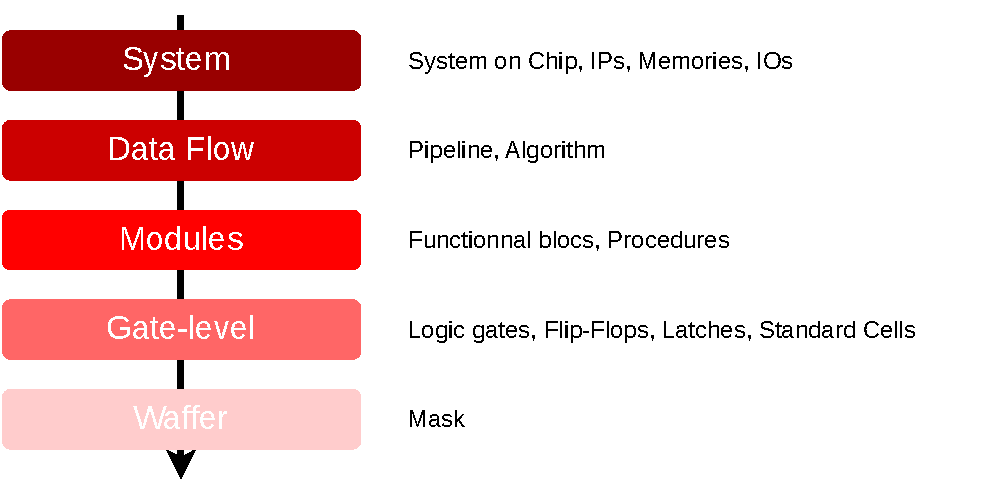
\includegraphics[width=\linewidth]{Figures/abstractions.pdf}
    \end{figure}
\end{frame}

\subsection{Combinational Logic}
\begin{frame}{Boolean Algebra}{\insertsection ~- \insertsubsection}
    \begin{columns}
        \column{0.65\textwidth}
        \begin{align}
            S &= \bar{A} \bar{B} {C_{in}} + \bar{A} {B} \bar{C_{in}} + {A} \bar{B} \bar{C_{in}} + {A} {B} {C_{in}} \label{eq:dnf_s}\\
            S &= A \oplus B \oplus {C_{in}} \\
            C_{out} &= \bar{A} {B} {C_{in}} + {A} \bar{B} {C_{in}} + A B \bar{C_{in}} + A B {C_{in}} \label{eq:dnf_cout}\\
            C_{out} &= A B + {C_{in}} ( A \oplus B)
        \end{align}

        \begin{boite1}{Note}
            \begin{itemize}
                \item (\ref{eq:dnf_s}) and (\ref{eq:dnf_cout}) are in Disjunctive Normal Form (DNF)
            \end{itemize}
        \end{boite1}

        \column{0.35\textwidth}
        \begin{table}[]
        \begin{tabular}{|ccc|cc|}
        \hline
        \multicolumn{3}{|c|}{Input}                              & \multicolumn{2}{c|}{Output}     \\ \hline
        \multicolumn{1}{|c|}{$A$} & \multicolumn{1}{c|}{$B$} & $C_{in}$ & \multicolumn{1}{c|}{$S$} & $C_{out}$ \\ \hline \hline
        0                       & 0                      & 0     & 0                      & 0      \\
        0                       & 0                      & 1     & 1                      & 0      \\
        0                       & 1                      & 0     & 1                      & 0      \\
        0                       & 1                      & 1     & 0                      & 1      \\
        1                       & 0                      & 0     & 1                      & 0      \\
        1                       & 0                      & 1     & 0                      & 1      \\
        1                       & 1                      & 0     & 0                      & 1      \\
        1                       & 1                      & 1     & 1                      & 1      \\ \hline
        \end{tabular}
        \end{table}
    \end{columns}
\end{frame}
\begin{frame}{Logic Gates}{\insertsection ~- \insertsubsection}
    \begin{figure}
        \centering
        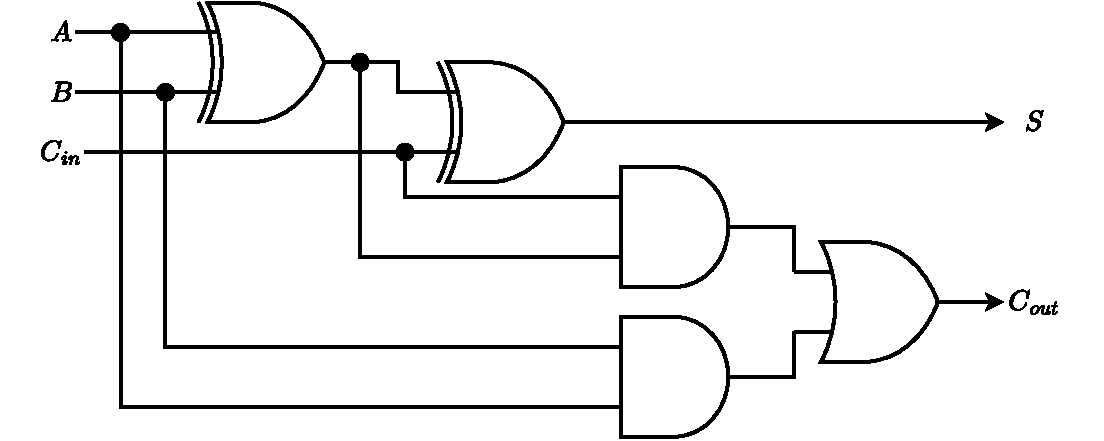
\includegraphics[width=\linewidth]{Figures/FA_gates.pdf}
    \end{figure}
\end{frame}
\begin{frame}{Transitor Implementation}{\insertsection ~- \insertsubsection}
    \begin{columns}[T]
        \column{0.3\textwidth}
            \begin{figure}
                \centering
                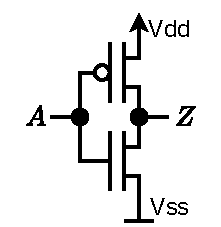
\includegraphics[scale=0.9]{Figures/trans_inverter.pdf}
            \end{figure}
            \vspace{1.2cm}
            \centering
            Inverter gate CMOS
        \column{0.3\textwidth}
            \begin{figure}
                \centering
                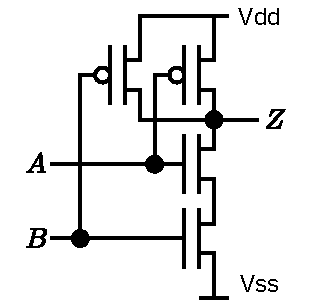
\includegraphics[scale=0.9]{Figures/trans_nand.pdf}
            \end{figure}
            \vfill
            \centering
            NAND gate CMOS
        \column{0.3\textwidth}
            \begin{figure}
                \centering
                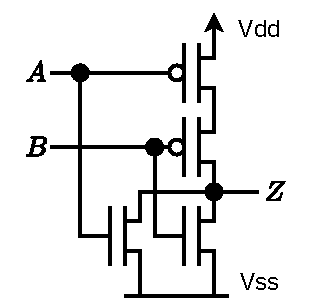
\includegraphics[scale=0.9]{Figures/trans_nor.pdf}
            \end{figure}
            \vfill
            \centering
            NOR gate CMOS
    \end{columns}
\end{frame}
\begin{frame}{Mask}{\insertsection ~- \insertsubsection}
    \begin{columns}
        \column{0.4\textwidth}
            \begin{figure}
                \centering
                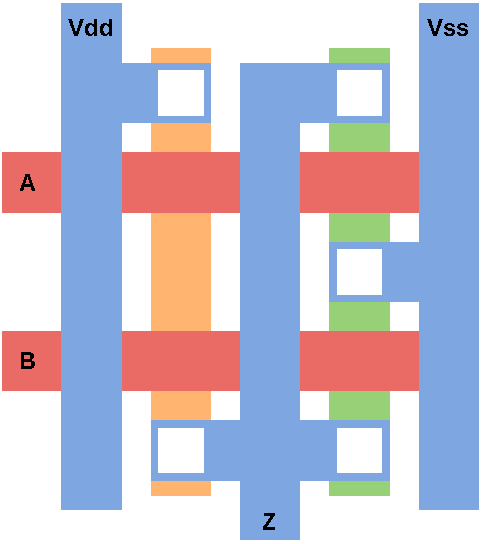
\includegraphics[scale=0.65]{Figures/mask_nor.pdf}
            \end{figure}
        \column{0.6\textwidth}
            \begin{columns}
                \column{0.2\columnwidth}
                    \begin{figure}
                        \centering
                        
\includegraphics[scale=0.65]{Figures/mask_metal.pdf}
                    \end{figure}
                \column{0.7\columnwidth}
                    \vspace{-0.35cm}
                    Metal
            \end{columns}
            \begin{columns}
                \column{0.2\columnwidth}
                    \begin{figure}
                        \centering
                        
\includegraphics[scale=0.65]{Figures/mask_poly.pdf}
                    \end{figure}
                \column{0.7\columnwidth}
                    \vspace{-0.35cm}
                    Gate (polysilicon)
            \end{columns}
                        \begin{columns}
                \column{0.2\columnwidth}
                    \begin{figure}
                        \centering
                        
\includegraphics[scale=0.65]{Figures/mask_diff_p.pdf}
                    \end{figure}
                \column{0.7\columnwidth}
                    \vspace{-0.35cm}
                    P diffusion
            \end{columns}
                        \begin{columns}
                \column{0.2\columnwidth}
                    \begin{figure}
                        \centering
                        
\includegraphics[scale=0.65]{Figures/mask_diff_n.pdf}
                    \end{figure}
                \column{0.7\columnwidth}
                    \vspace{-0.35cm}
                    N diffusion
            \end{columns}
    \end{columns}
\end{frame}


\section{Design Families}
\subsection{Overview}
\begin{frame}{\insertsubsection}{\insertsection}
   % Frame with Flexibility vs Performance Figure

    \begin{figure}
        \centering
        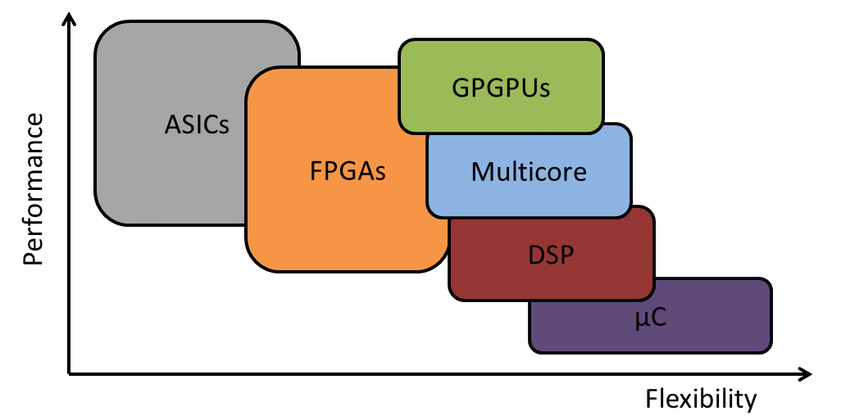
\includegraphics[width=.9\textwidth]{Figures/Performance-vs-Flexibility.png}
        \caption{Performance vs Flexibility \cite{article}}
    \end{figure}

\end{frame}

\subsection{Central Processing Unit}
\begin{frame}{Instruction Set Architecture}{\insertsection ~- \insertsubsection}
    % Present ISA and programs
    % Present SISD
    \begin{columns}
        \column{0.42\textwidth}
        \begin{itemize}
            \item Instruction Set Architecture (ISA)
            \item Single Instruction Single Data (SISD)
            \item Executes a program stored in memory
        \end{itemize}

        \column{0.6\textwidth}
        \begin{figure}
            \centering
            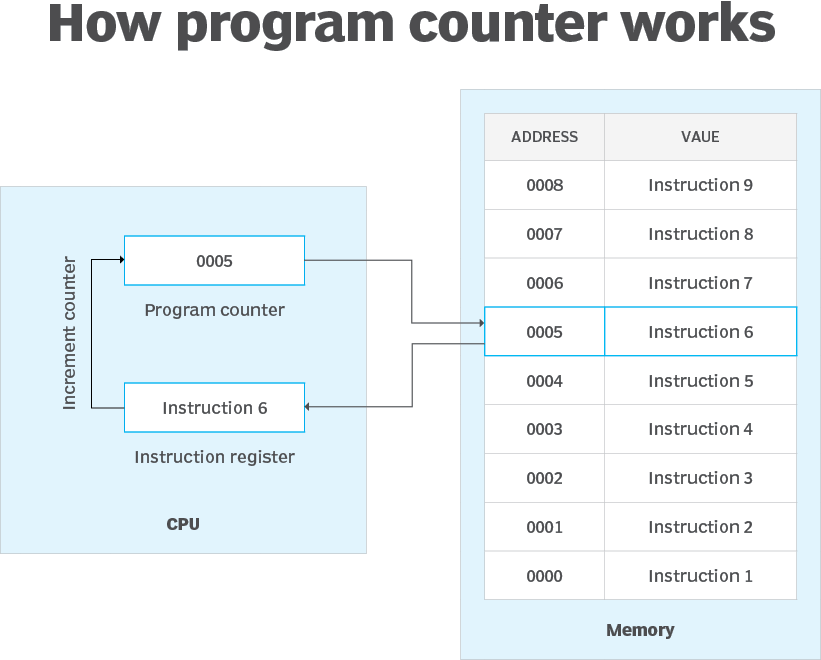
\includegraphics[width=.9\textwidth]{Figures/how_program_counter_works.png}
            \caption{Program \cite{noauthor_what_nodate}}
        \end{figure}
        % Figure
    \end{columns}
\end{frame}

\begin{frame}{Von Neumann \& Harvard Architecture}{\insertsection ~- \insertsubsection}
    % Compare the system view of Van Neumann and Harvard
    % Main Components (IO, Memory, Execution)
    \begin{columns}
        \column{0.49\textwidth}
        \begin{figure}
            \centering
            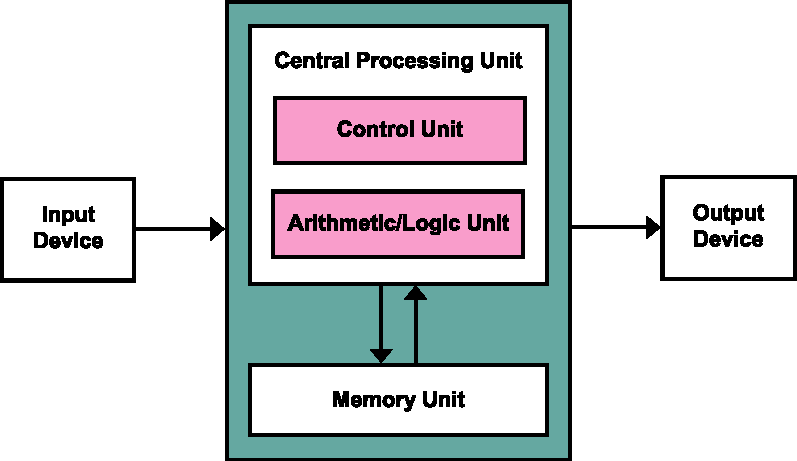
\includegraphics[width=\textwidth]{Figures/Von_Neumann_Architecture.pdf}
            \caption{Von Neumann Architecture \cite{noauthor_von_2025}}
        \end{figure}

        \column{0.49\textwidth}
        \begin{figure}
            \centering
            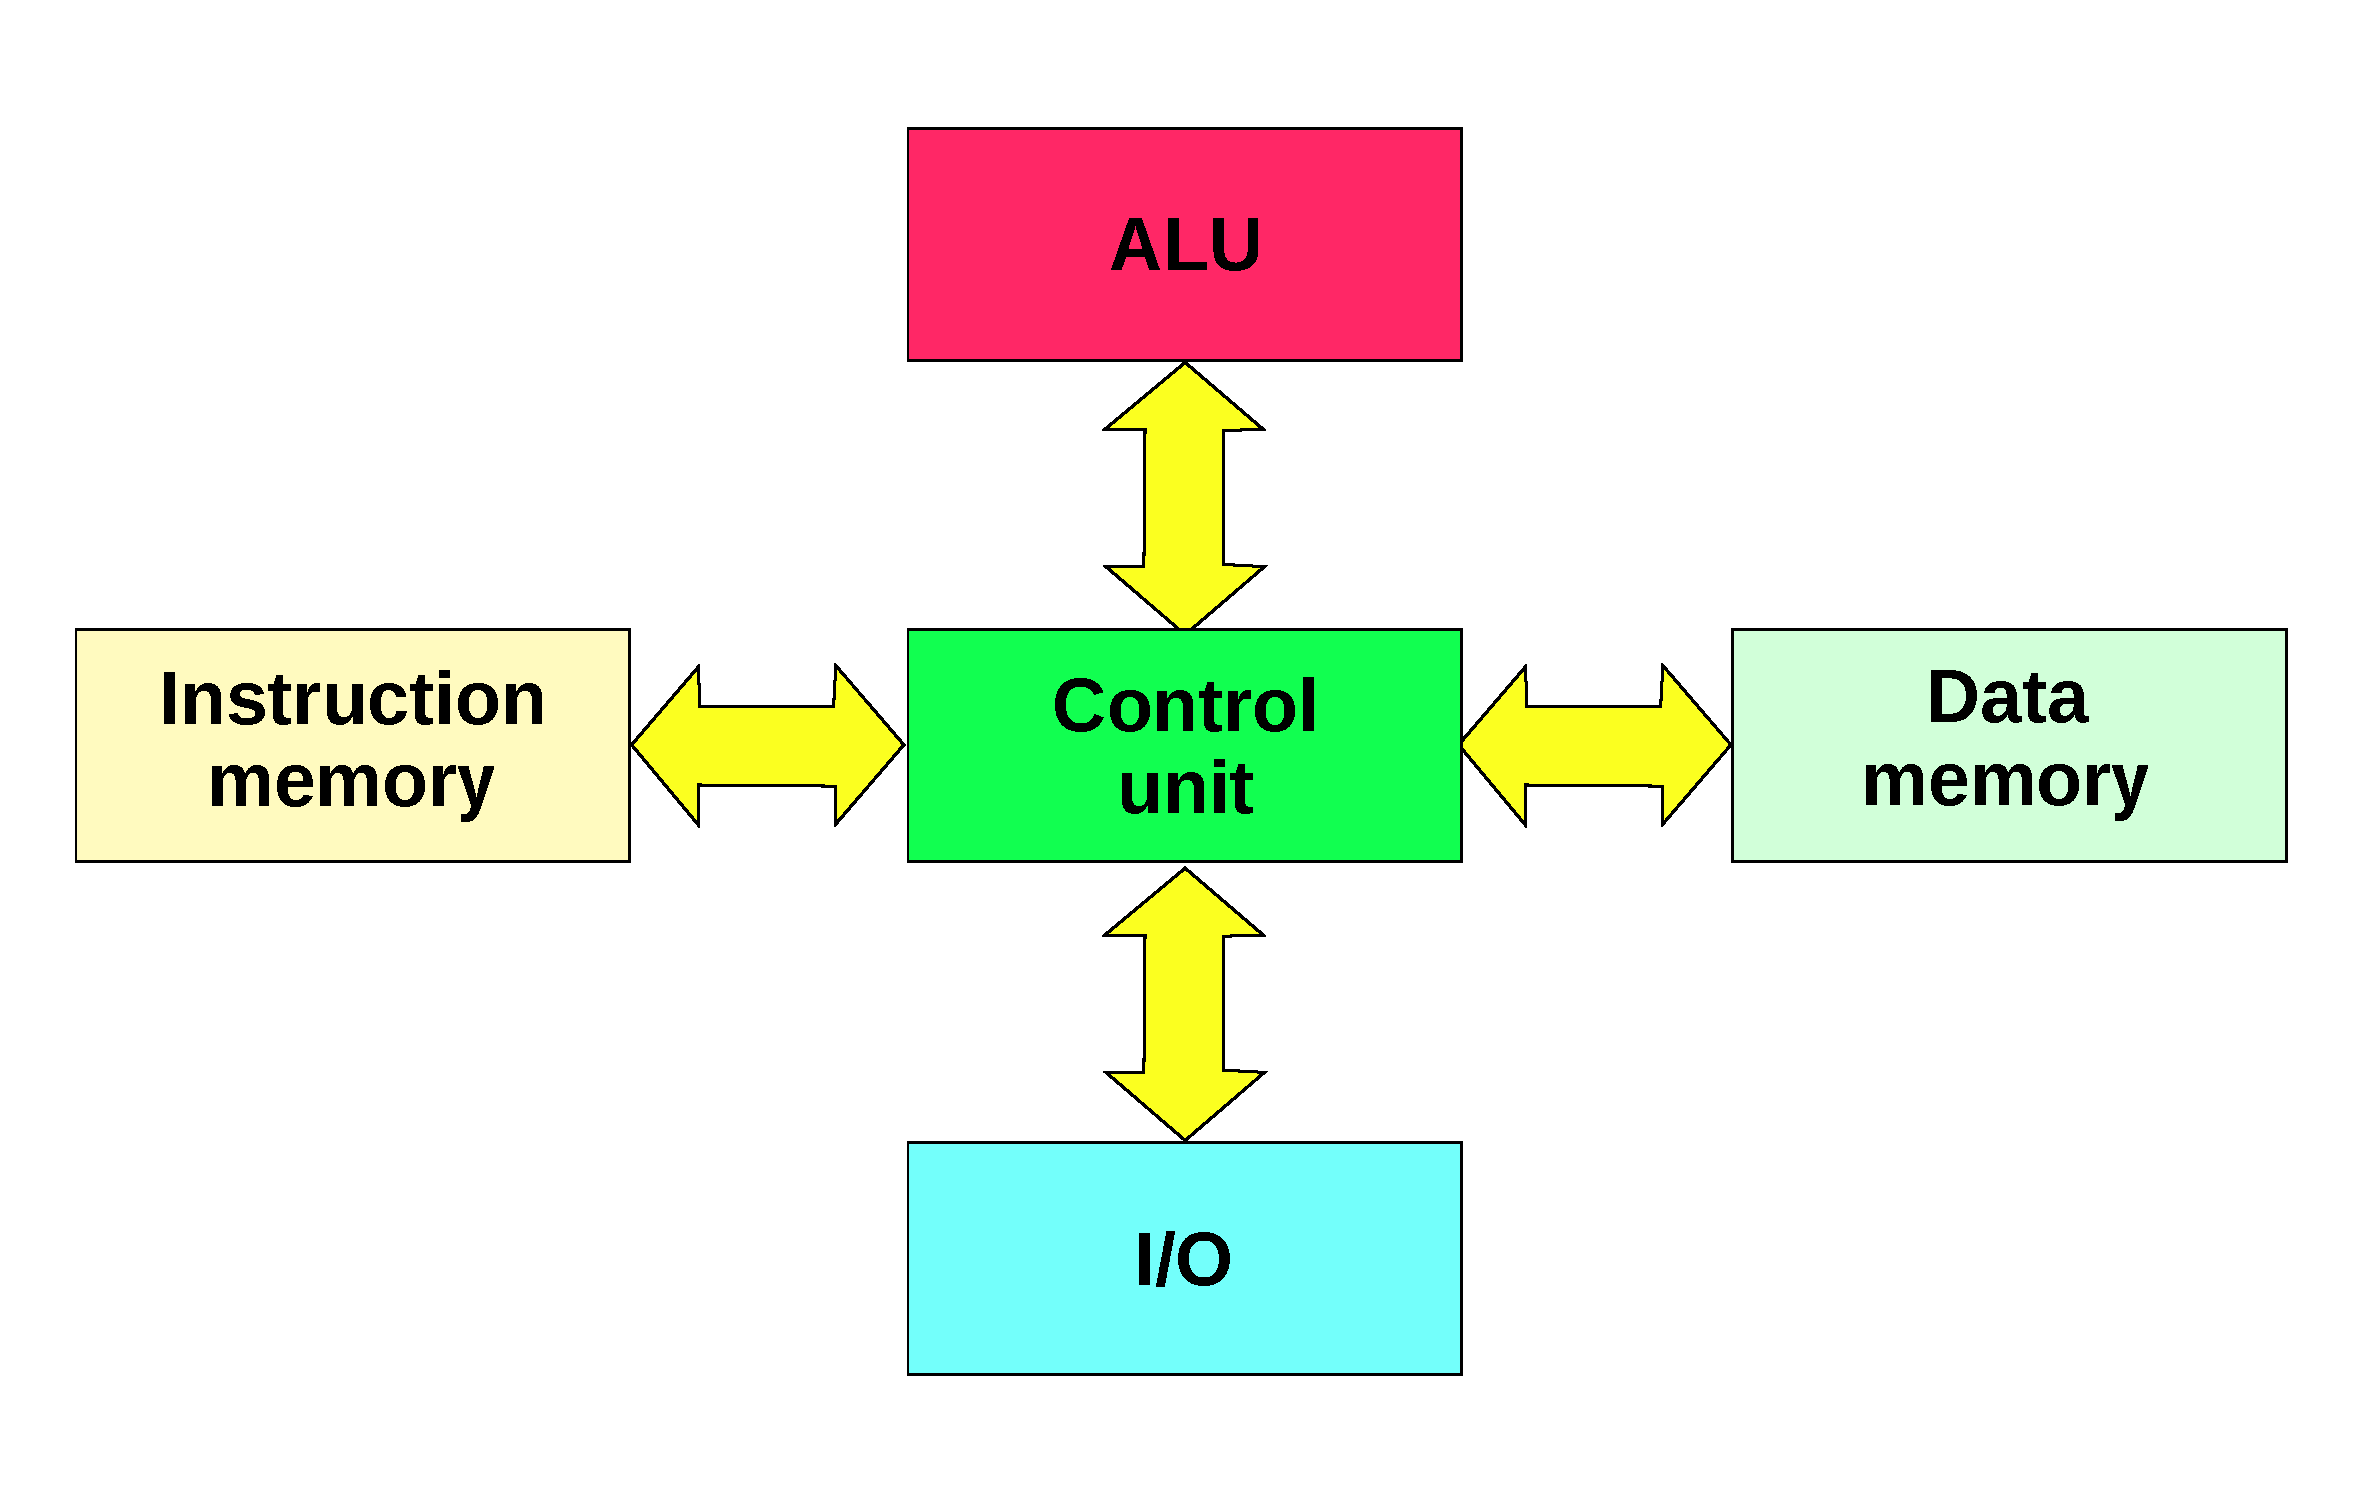
\includegraphics[width=\textwidth]{Figures/Harvard_architecture.pdf}
            \caption{Harvard Architecture \cite{noauthor_harvard_2025}}
        \end{figure}
    \end{columns}
\end{frame}

\begin{frame}{Execution Pipeline}{\insertsection ~- \insertsubsection}
    % Present the 5 stage execution pipeline
    \begin{columns}
        \column{0.4\textwidth}
        Stages :
        \begin{itemize}
            \item IF: Instruction Fetch
            \item ID: Instruction Decode
            \item EX: Execute
            \item MEM: Memory access
            \item WB: WriteBack
        \end{itemize}

        \column{0.6\textwidth}
        \begin{figure}
            \centering
            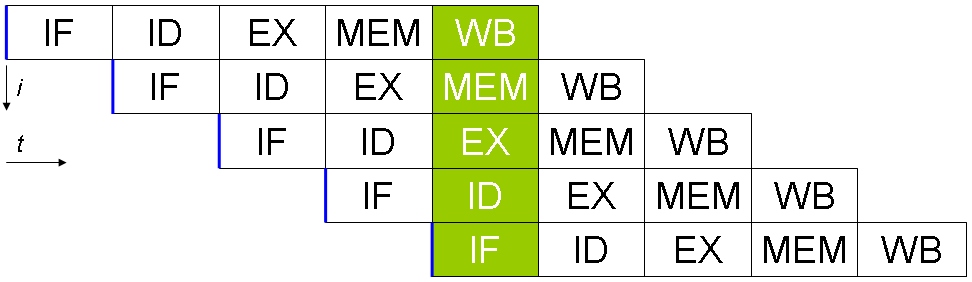
\includegraphics[width=\textwidth]{Figures/Fivestagespipeline.png}
            \caption{Five stage pipeline \cite{noauthor_classic_2025}}
        \end{figure}
    \end{columns}
\end{frame}

\subsection{Graphical Processing Unit}
\begin{frame}{Single Instruction Multiple Data}{\insertsection ~- \insertsubsection}
    % Present SIMD
    % Present vector computation
    \begin{columns}
        \column{0.49\textwidth}
        \begin{itemize}
            \item Single Instruction Multiple Data (SIMD)
            \item Vector operations
            \begin{itemize}
                \item e.g. scalar multiplication $a\vec{v}$
            \end{itemize}
        \end{itemize}

        \column{0.5\textwidth}
        \begin{figure}
            \centering
            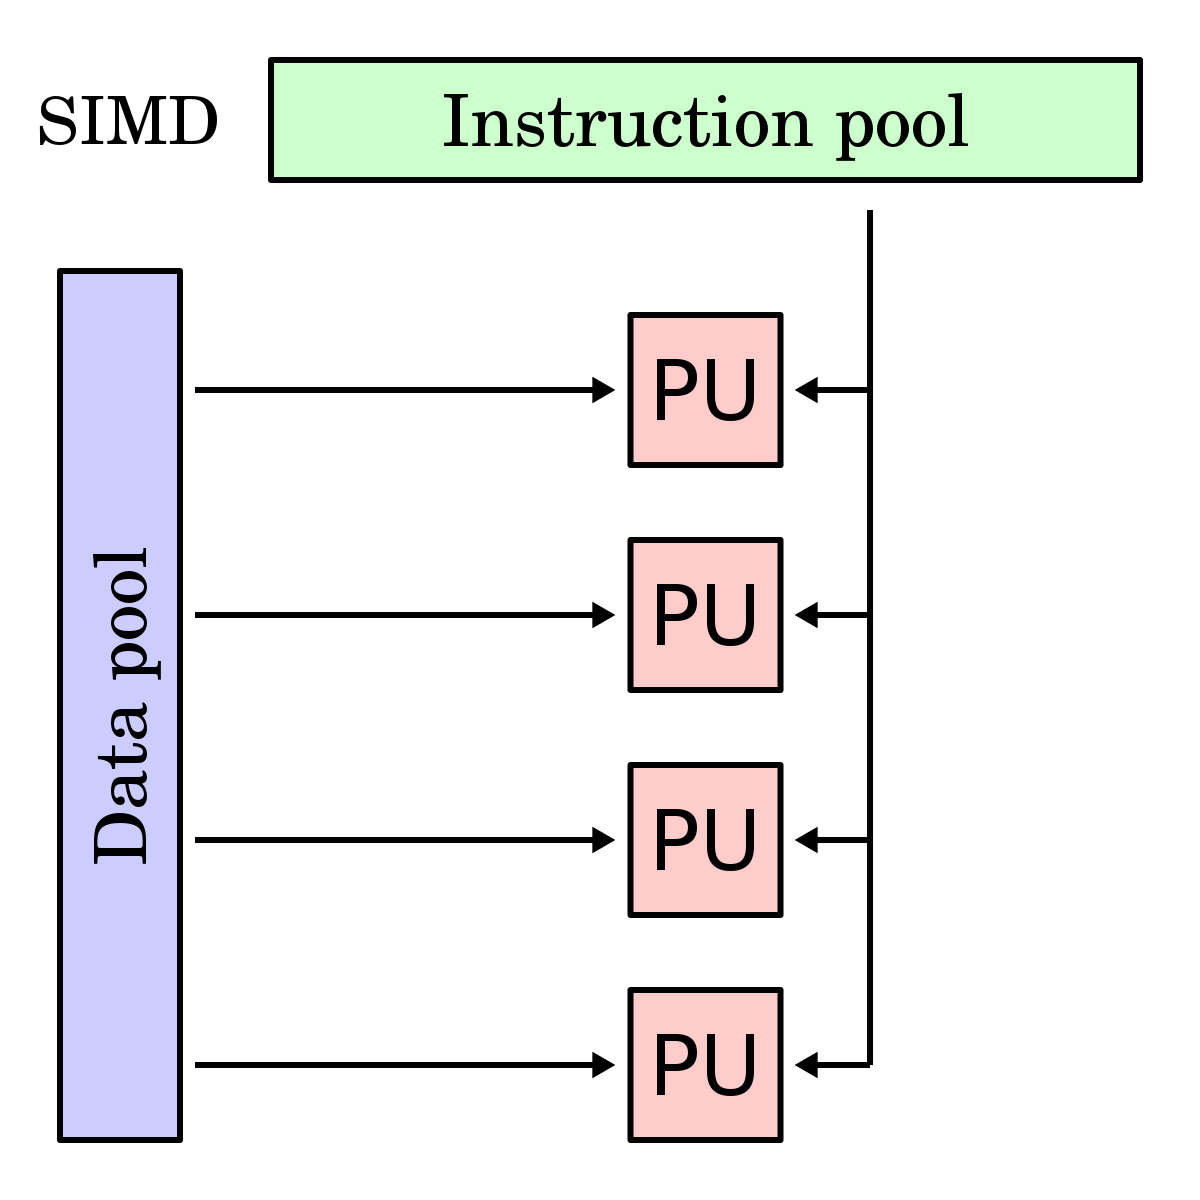
\includegraphics[width=.85\textwidth]{Figures/simd.png}
            \caption{Instruction to Processing Unit (PU) \cite{noauthor_simd_nodate}}
        \end{figure}
    \end{columns}
\end{frame}

\begin{frame}{Parallel vs Serial}{\insertsection ~- \insertsubsection}
    \centering
    Multiply ACcumulation (MAC) operation in dot product $\vec{a} \cdot \vec{b}$
    % Compare implementations in term of performance, area, latency etc
    % Present a MAC as an example ?
    \begin{columns}[T]
        \column{0.49\textwidth}
        \centering
        Serial:
        % \vspace{1.8cm}
        \begin{figure}
            \centering
            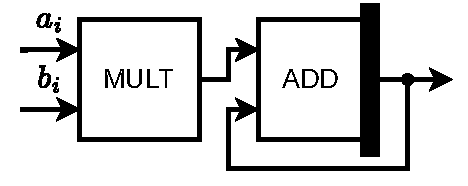
\includegraphics[scale=0.55]{Figures/serial.pdf}
        \end{figure}
        \begin{boite1}{Comparison}
            \begin{itemize}
                \item Size
                \item Power consumption
                \item Latency
            \end{itemize}
        \end{boite1}

        \column{0.49\textwidth}
        \centering
        Parallel:
        \begin{figure}
            \centering
            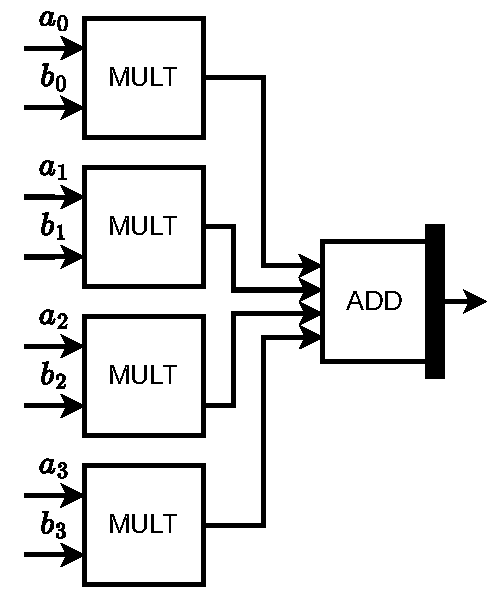
\includegraphics[scale=0.55]{Figures/parallel.pdf}
        \end{figure}
    \end{columns}
\end{frame}

\subsection{Field-Programmable Gate Array \cite{noauthor_what_2024}}
\begin{frame}{\insertsubsection}{\insertsection}
    % Present reconfigurable hardware
    % Present LUT architecture
    \begin{columns}[c]
        \column{0.49\textwidth}
        \centering
        % \vspace{1.8cm}
        \begin{figure}
            \centering
            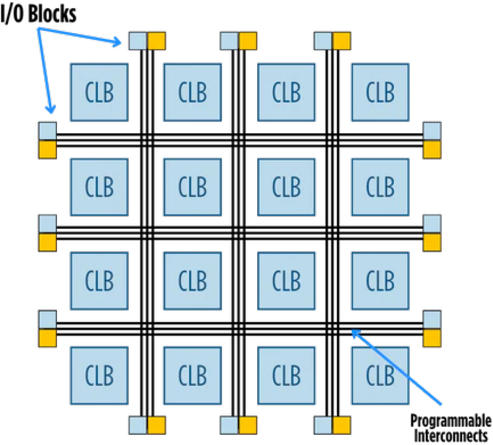
\includegraphics[width=\textwidth]{Figures/fpga_board.pdf}
        \end{figure}

        \column{0.49\textwidth}
        \centering
        \begin{figure}
            \centering
            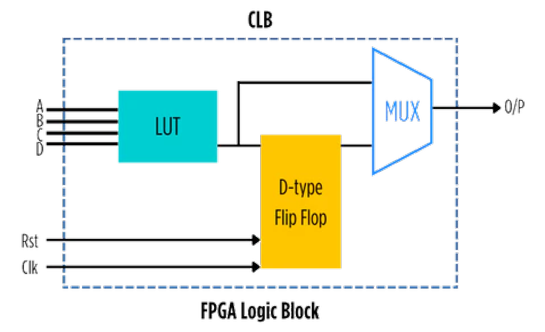
\includegraphics[width=\textwidth]{Figures/fpga_CLB.pdf}
        \end{figure}
    \end{columns}
\end{frame}

\subsection{System on Chip}
\begin{frame}{\insertsubsection}{\insertsection}
    % Present a computing platform with a bus, Peripheral bridge and memories
    \begin{figure}
        \centering
        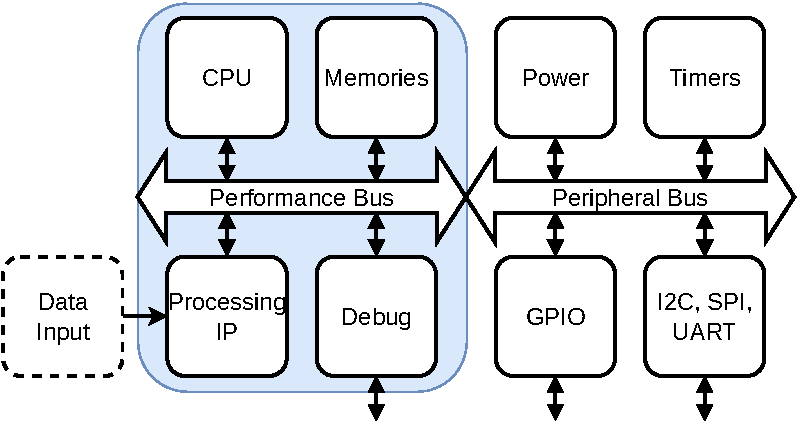
\includegraphics[width=.9\textwidth]{Figures/system_bus.pdf}
    \end{figure}
\end{frame}

% \subsection{Application-Specific Integrated Circuit \& IPs}
% \begin{frame}{\insertsubsection}{\insertsection}
%     % System on Chip with IPs
%     % Multi-abstraction level design
%     \begin{columns}[c]
%         \column{0.49\textwidth}
%         \centering
%         \textbf{Application-Specific Integrated Circuit (ASIC)}
%         \begin{itemize}
%             \item Covers the whole design flow
%         \end{itemize}

%         \column{0.49\textwidth}
%         \centering
%         \begin{figure}
%             \centering
%             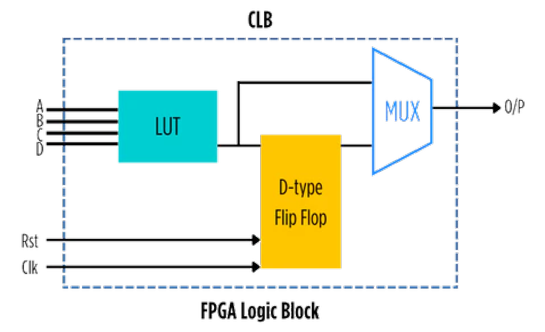
\includegraphics[width=\textwidth]{Figures/fpga_CLB.pdf}
%         \end{figure}
%     \end{columns}
% \end{frame}

\section{Design Flow}

\subsection{Successive Refinement}
\begin{frame}{Gajski-Kuhn chart}{\insertsection ~- \insertsubsection}
    % Present Y chart and spiral steps
    \begin{columns}[c]
        \column{0.49\textwidth}
        \centering
        % \vspace{1.8cm}
        \begin{figure}
            \centering
            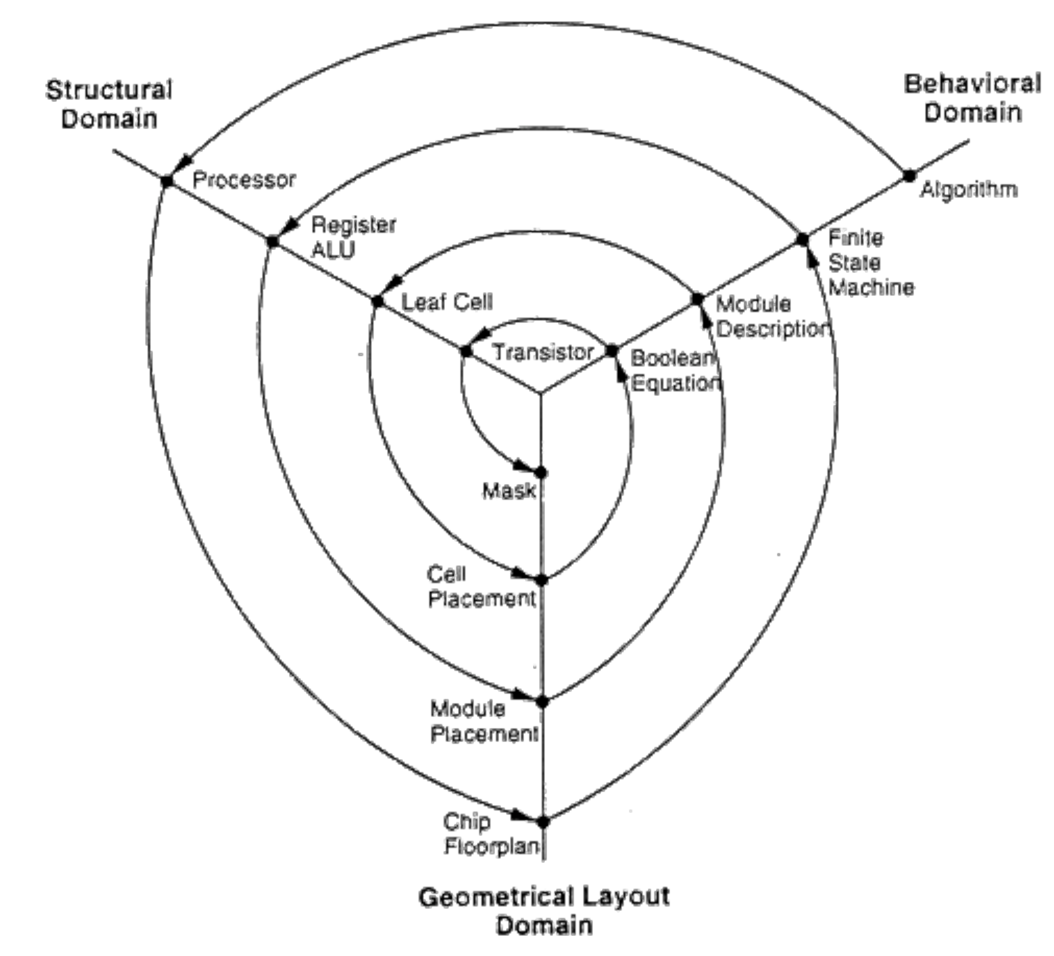
\includegraphics[width=\textwidth]{Figures/y_chart.pdf}
        \end{figure}

        \column{0.49\textwidth}
        \begin{boite1}{Perspectives}
        \begin{itemize}
            \item Behavioral
            \item Structural
            \item Physical/Geometry
        \end{itemize}
        \end{boite1}

        \textbf{Logical synthesis} : from behavioral to structural

        \textbf{Physical synthesis / Layout} : from structural to physical / geometrical

    \end{columns}
\end{frame}

\begin{frame}{Front-End Flow}{\insertsection ~- \insertsubsection}
    % Present HLS and Logic Synthesis
    \begin{columns}[T]
        \column{0.49\textwidth}
        \centering
        \textbf{High Level Synthesis}
        \begin{itemize}
            \item From a system-level description
            \item Produces a Finite State Machine (FSM)
            \item Followed by logical synthesis
        \end{itemize}

        \column{0.49\textwidth}
        \centering
        \textbf{Logical synthesis}
        \begin{itemize}
            \item Takes a RTL description (e.g. FSM) \& technology node
            \item Builds a abstract representation of the logic and maps it to standard cell
            \item Produces a netlist / gate-level circuit
        \end{itemize}
    \end{columns}
\end{frame}

\begin{frame}{Back-End Flow}{\insertsection ~- \insertsubsection}
    % Present Floor plan, Place and Route
    \begin{columns}[c]
        \column{0.39\textwidth}
        Steps :
        \begin{itemize}
            \item Partitioning
            \item Floorplanning
            \item Placement
            \item Global routing
            \item Detailed routing
        \end{itemize}

        \column{0.59\textwidth}
        \begin{figure}
            \centering
            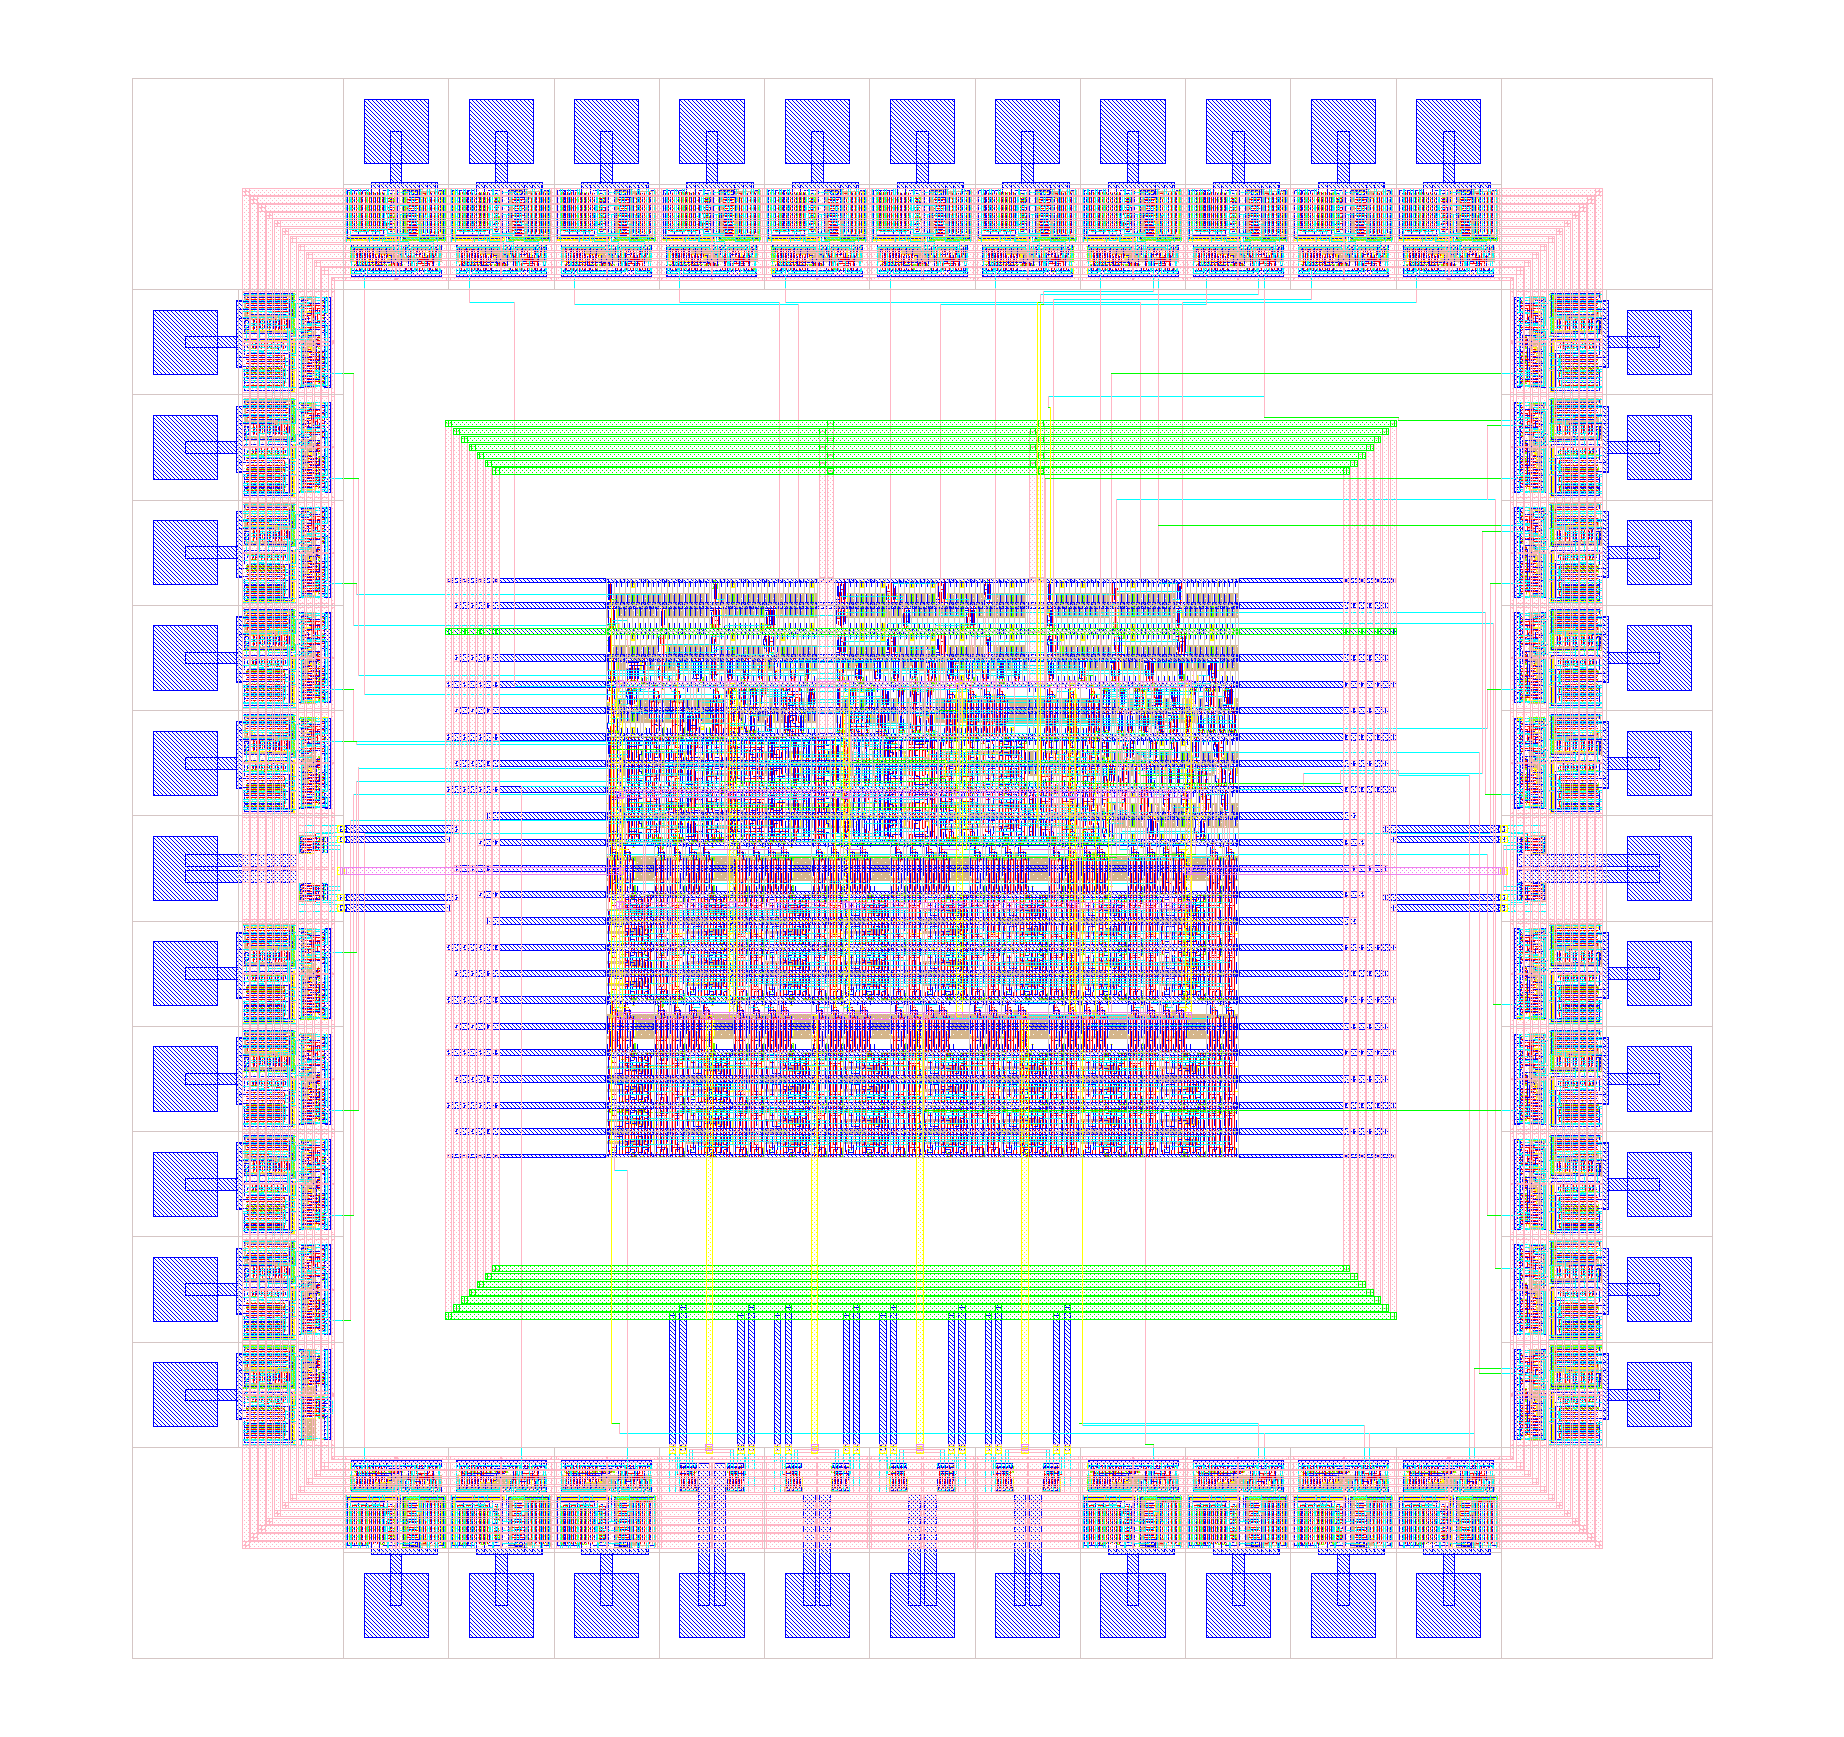
\includegraphics[width=.8\textwidth]{Figures/amd2901_chip_routed.png}
            \caption{Chip layout \cite{noauthor_coriolis_nodate}}
        \end{figure}
    \end{columns}
\end{frame}

\subsection{Verification \& Validation}
\begin{frame}{\insertsubsection}{\insertsection}
    % Present Testbench, golden, different types of simulation
    \begin{columns}[c]
        \column{0.39\textwidth}
        \begin{boite1}{Verification}
            \begin{itemize}
                \item Functional Simulation
                \begin{itemize}
                    \item Behavioral
                    \item Gate-level (Timed)
                    \item Analog
                \end{itemize}
                \item Formal Verification
            \end{itemize}
        \end{boite1}

        \begin{boite}{Validation}
            \begin{itemize}
                \item FPGA (Behavioral)
                \item Static Timing Analysis and Timing Closure
            \end{itemize}
        \end{boite}

        % \begin{boite1}{Formal Verification}
        %     \begin{itemize}
        %         \item
        %     \end{itemize}
        % \end{boite1}

        \column{0.5\textwidth}
        \begin{figure}
            \centering
            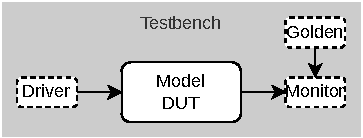
\includegraphics[width=.85\textwidth]{Figures/testbench_model.pdf}
            \caption{Simulated Testbench}
        \end{figure}

        \begin{figure}
            \centering
            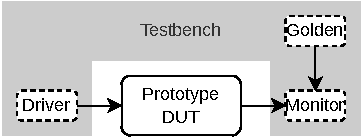
\includegraphics[width=.85\textwidth]{Figures/testbench_hil.pdf}
            \caption{Hardware in the loop}
        \end{figure}
    \end{columns}

\end{frame}

% \begin{frame}{Prototype}{\insertsection ~- \insertsubsection}
%     % Present FPGA and so on
% \end{frame}

% \begin{frame}{Formal Verification}{\insertsection ~- \insertsubsection}
%     % Present KMA stuff
% \end{frame}

\section*{Summary}
\begin{frame}{\insertsection}
 \begin{itemize}
    \item The IC design flow consist of successive refinement accross abstraction layers
    \item Design choices : Flexibility vs Performance, Serial vs Parallel, etc.
    \item CPUs and GPUs are instruction set architectures that execute programs
    \item System on chip are composed of multiple subsystems (IPs)
    \item FPGA are a good platform to prototype hardware designs
 \end{itemize}
\end{frame}